\subsubsection{Administrationsbereich}
\label{sec:Administrationsbereich}

Ein Oberflächenentwurf des Administrationsbereiches ist in
\abbildung{MockupBackend} dargestellt.

\begin{figure}[htb]
\centering
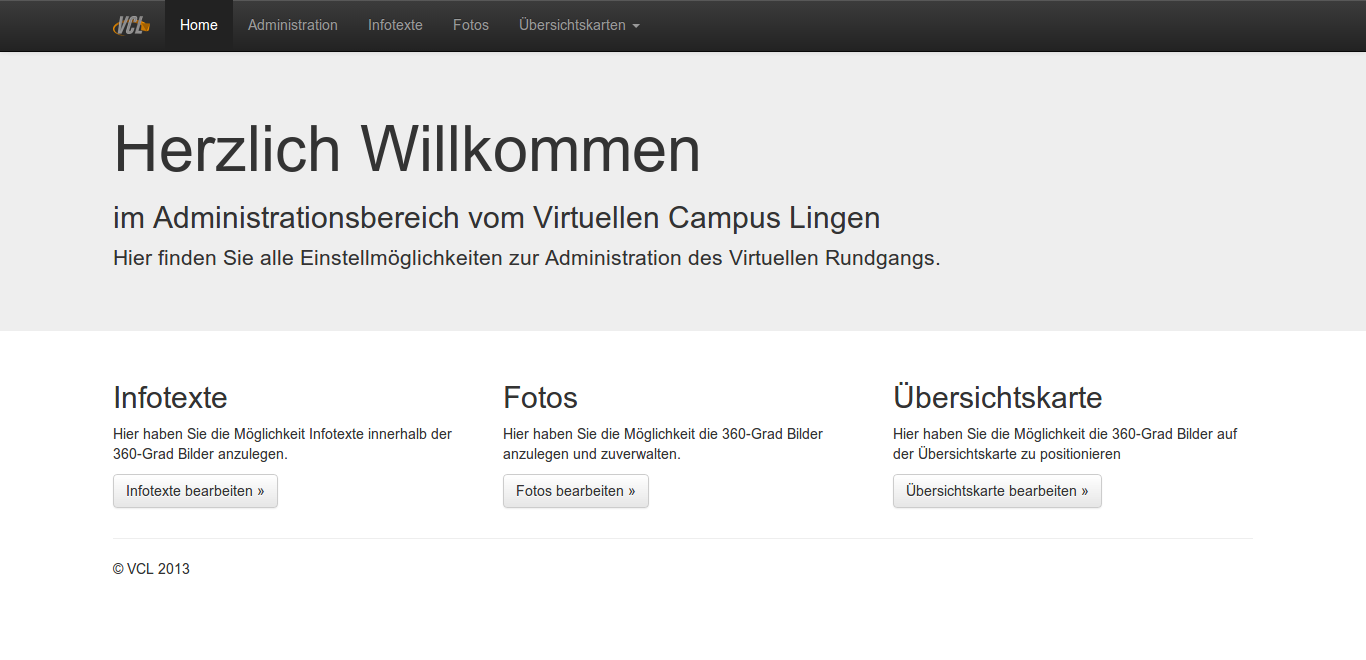
\includegraphics[width=1.0\textwidth]{MockupBackend.png}
\caption[Oberflächenentwurf des
Administrationsbereiches]{Oberflächenentwurf des
Administrationsbereiches\protect\footnotemark}
\label{fig:MockupBackend}
\end{figure}
\footnotetext{Quelle: Eigene Darstellung}

Der Administartionsbereich gliedert sich hierbei in folgende Bereiche:

\begin{itemize}
  \item Infotextverwaltung
  \item Fotoverwaltung
  \item Interessante Ort
  \item Übersichtskarte
\end{itemize}

In der \textbf{Infotextverwaltung} können Informationstexte verfasst und zu
Panoramafotos zugeordnet werden. Ein Informationstext kann dabei auch mehreren
Fotos zugeordnet werden. Dadurch können dem Benutzer alle Informationstexte
angezeigt werden, die sich auf den Standpunkt beziehen, an dem sich dieser
gerade befindet. Alle Informationstexte, die bereits erstellt wurden, werden in
der Infotextverfaltung tabellarisch aufgelistet. Jeder dieser Informationstexte
kann sowohl verändert als auch gelöscht werden.

In der \textbf{Fotoverwaltung} werden analog zu der Infotextverwaltung die
erstellten Panoramafotos hinterlegt und gepflegt. Erstellte Panoramafotos
können in diesem Menüpunkt mit Namen und Beschreibung hochgeladen werden.
Analog zu den Infotexten werden hier die bereits hochgeladenen Fotos
tabellarisch aufgelistet. Auch die Möglichkeit zur Änderung und Löschung der
Fotos ist hier gegeben.

Der Bereich \textbf{Interessante Orte} bietet die
Möglichkeit, die Standorte zu hinterlegen, die dem Benutzer beim Klicken
auf die Minimap angezeigt werden. Zu diesen Standorten kann der Benutzer
dann springen, ohne dorthin navigieren zu müssen. Diese Möglichkeit ist vorallem
für Benutzer der Anwendung von Vorteil, die den Campus nicht kennen und nicht
erst nach bestimmten Orten suchen wollen. Zur Pflege der interessanten Orte muss
im entsprechenden Bereich in der Administrationsoberfläche nur ein
beschreibender Text eingetragen und mit einem hochgeladenen Foto verlinkt werden.
 
Die \textbf{Übersichtskarte} stellt den letzten und komplexesten Bereich des
Administrationsbereiches dar. In der Übersichtskarte werden die hochgeladenen
Panoramafotos auf einer Karte des Hochschulgebäudes platziert. Dazu wird dem
angemeldeten Administrator zunächst eine topographische Karte des Campus
präsentiert. Auf dieser Karte kann der Administrator durch Klicken eine
Position bestimmen, zu der er ein Foto auswählen und speichern kann.
Ein Foto kann dabei nur an einer Position auf der Übersichtskarte platziert
werden. Der Administrator hat die Möglichkeit die Position jedes Fotos beliebig
oft zu ändern. Darüber hinaus werden dem Administrator Steuerelemente angezeigt
mit denen er einen bestimmten Bereich des Campus auswählen kann, in dem er
Fotos positionieren möchte. So kann der Administrator sowohl zwischen
verschiedenen Gebäudekomplexen als auch zwischen den einzelnen Stockwerken
innerhalb eines Gebäudekomplexes wählen. Neben der Möglichkeit ein Foto zu
positionieren hat der Administrator weiterhin die Möglichkeit die Verbindungen
zwischen positionierten Fotos zu pflegen. Aus dem Oberflächenentwurf der
Benutzeroberfläche, welcher im vorherigen Abschnitt vorgestellt wurde, ist
ersichtlich, dass ein Benutzer von einem Panoramafoto aus zu einem anderen
Standpunkt navigieren kann. Diese Navigation beruht auf Verbindungen zwischen
den Panoramafotos. Solche Verbindungen werden in der Übersichtskarte gepflegt.
Die Steuerungselemente zu Pflege der Verbindungen zwischen Panoramafotos sind zum
Zeitpunkt der Erstellung des Mockups noch nicht definiert, die Notwendigkeit
dieser Funktion ist aber bedacht.